\documentclass[a5paper, 10pt]{article}

% Текст
\usepackage[utf8]{inputenc} % UTF-8 кодировка
\usepackage[russian]{babel} % Русский язык
\usepackage{indentfirst} % красная строка в первом параграфе в главе
% Отображение страниц
\usepackage{geometry} % размеры листа и отступов
\usepackage{listings}
\usepackage{color}

\usepackage{float}
\floatplacement{figure}{H}

\geometry{
	left=12mm,
	top=25mm,
	right=15mm,
	bottom=17mm,
	marginparsep=0mm,
	marginparwidth=0mm,
	headheight=10mm,
	headsep=7mm,
	nofoot}
\usepackage{afterpage,fancyhdr} % настройка колонтитулов
\pagestyle{fancy}
\fancypagestyle{style}{ % создание нового стиля style
	\fancyhf{} % очистка колонтитулов
	\fancyhead[LO, RE]{ЛР № 3 } % название документа наверху
	\fancyhead[RO, LE]{Вынужденное движение и показатели качества} % название section наверху
	\fancyfoot[RO, LE]{\thepage} % номер страницы справа внизу на нечетных и слева внизу на четных
	\renewcommand{\headrulewidth}{0.25pt} % толщина линии сверху
	\renewcommand{\footrulewidth}{0pt} % толцина линии снизу
}
\fancypagestyle{plain}{ % создание нового стиля plain -- полностью пустого
	\fancyhf{}
	\renewcommand{\headrulewidth}{0pt}
}
\fancypagestyle{title}{ % создание нового стиля title -- для титульной страницы
	\fancyhf{}
	\fancyhead[C]{{\footnotesize
			Министерство образования и науки Российской Федерации\\
			Федеральное государственное автономное образовательное учреждение высшего образования
	}}
	\fancyfoot[C]{{\large 
			Санкт-Петербург, 2026
	}}
	\renewcommand{\headrulewidth}{0pt}
}

%Программирование
\usepackage{listings}

\definecolor{codegreen}{rgb}{0,0.6,0}
\definecolor{codegray}{rgb}{0.5,0.5,0.5}
\definecolor{codepurple}{rgb}{0.58,0,0.82}
\definecolor{backcolour}{rgb}{0.95,0.95,0.92}

\lstdefinestyle{codestyle}{
    backgroundcolor=\color{backcolour},
    keywordstyle=\color{magenta},
    numberstyle=\tiny\color{codegray},
    stringstyle=\color{codepurple},
    basicstyle=\ttfamily\footnotesize,
    breakatwhitespace=false,
    breaklines=true,
    captionpos=b,
    keepspaces=true,
    numbers=left,
    numbersep=5pt,
    showspaces=false,
    showstringspaces=false, % показывать или нет пробелы специальными отступами
    showtabs=false, % показывать или нет табуляцию в строках
    tabsize=2 % размер табуляции по умолчанию равен 2 пробелам
}
\lstset{
    language=Python, % Язык программирования
    basicstyle=\ttfamily\small, % Стиль текста
    commentstyle=\color{green}, % Стиль комментариев
    keywordstyle=\color{blue}, % Стиль ключевых слов
    stringstyle=\color{red}, % Стиль строк
    showstringspaces=false, % Не показывать пробелы в строках
    breaklines=true, % Переносить длинные строки
    extendedchars=true, % Поддержка кириллицы
    inputencoding=utf8, % Кодировка входного файла
    numbers=left,               % где поставить нумерацию строк (слева\справа)
    numberstyle=\tiny,           % размер шрифта для номеров строк
    stepnumber=1,                   % размер шага между двумя номерами строк
    numbersep=5pt,                % как далеко отстоят номера строк от подсвечиваемого кода
    captionpos=b,              % позиция заголовка вверху [t] или внизу [b] 
    breaklines=true,           % автоматически переносить строки (да\нет)
    breakatwhitespace=false, % переносить строки только если есть пробел
    literate={а}{{\cyra}}1 {б}{{\cyrb}}1 {в}{{\cyrv}}1 {г}{{\cyrg}}1 {д}{{\cyrd}}1
             {е}{{\cyre}}1 {ё}{{\cyryo}}1 {ж}{{\cyrzh}}1 {з}{{\cyrz}}1 {и}{{\cyri}}1
             {й}{{\cyrishrt}}1 {к}{{\cyrk}}1 {л}{{\cyrl}}1 {м}{{\cyrm}}1 {н}{{\cyrn}}1
             {о}{{\cyro}}1 {п}{{\cyrp}}1 {р}{{\cyrr}}1 {с}{{\cyrs}}1 {т}{{\cyrt}}1
             {у}{{\cyru}}1 {ф}{{\cyrf}}1 {х}{{\cyrh}}1 {ц}{{\cyrc}}1 {ч}{{\cyrch}}1
             {ш}{{\cyrsh}}1 {щ}{{\cyrshch}}1 {ъ}{{\cyrhrdsn}}1 {ы}{{\cyrery}}1
             {ь}{{\cyrsftsn}}1 {э}{{\cyrerev}}1 {ю}{{\cyryu}}1 {я}{{\cyrya}}1
             {А}{{\CYRA}}1 {Б}{{\CYRB}}1 {В}{{\CYRV}}1 {Г}{{\CYRG}}1 {Д}{{\CYRD}}1
             {Е}{{\CYRE}}1 {Ё}{{\CYRYO}}1 {Ж}{{\CYRZH}}1 {З}{{\CYRZ}}1 {И}{{\CYRI}}1
             {Й}{{\CYRISHRT}}1 {К}{{\CYRK}}1 {Л}{{\CYRL}}1 {М}{{\CYRM}}1 {Н}{{\CYRN}}1
             {О}{{\CYRO}}1 {П}{{\CYRP}}1 {Р}{{\CYRR}}1 {С}{{\CYRS}}1 {Т}{{\CYRT}}1
             {У}{{\CYRU}}1 {Ф}{{\CYRF}}1 {Х}{{\CYRH}}1 {Ц}{{\CYRC}}1 {Ч}{{\CYRCH}}1
             {Ш}{{\CYRSH}}1 {Щ}{{\CYRSHCH}}1 {Ъ}{{\CYRHRDSN}}1 {Ы}{{\CYRERY}}1
             {Ь}{{\CYRSFTSN}}1 {Э}{{\CYREREV}}1 {Ю}{{\CYRYU}}1 {Я}{{\CYRYA}}1,
}

\lstset{style=codestyle}

% Математика
\usepackage{amsmath, amsfonts, amssymb, amsthm} % Набор пакетов для математических текстов
%\usepackage{dmvnbase} % мехматовский пакет latex-сокращений
\usepackage{cancel} % зачеркивание для сокращений
% Рисунки и фигуры
\usepackage[pdftex]{graphicx} % вставка рисунков
\usepackage{wrapfig, subcaption} % вставка фигур, обтекая текст
\usepackage{caption} % для настройки подписей
\captionsetup{figurewithin=none,labelsep=period, font={small,it}} % настройка подписей к рисункам
% Рисование
\usepackage{tikz} % рисование
\usepackage{circuitikz}
\usepackage{pgfplots} % графики
% Таблицы
\usepackage{multirow} % объединение строк
\usepackage{multicol} % объединение столбцов
% Остальное
%\usepackage[unicode, pdftex]{hyperref} % гиперссылки
\usepackage[colorlinks]{hyperref} % гиперссылки
\hypersetup{
    linkcolor=blue,
    filecolor=magenta,
    urlcolor=cyan
}
\usepackage{enumitem} % нормальное оформление списков
\setlist{itemsep=0.15cm,topsep=0.15cm,parsep=1pt} % настройки списков
% Теоремы, леммы, определения...
\theoremstyle{definition}
\newtheorem{Def}{Определение}
\newtheorem*{Axiom}{Аксиома}
\theoremstyle{plain}
\newtheorem{Th}{Теорема}
\newtheorem{Lem}{Лемма}
\newtheorem{Cor}{Следствие}
\newtheorem{Ex}{Пример}
\theoremstyle{remark}
\newtheorem*{Note}{Замечание}
\newtheorem*{Solution}{Решение}
\newtheorem*{Proof}{Доказательство}
% Свои команды
\newcommand{\comb}[1]{\left[\hspace{-4pt}\begin{array}{l}#1\end{array}\right.\hspace{-5pt} } % совокупность уравнений
% Титульный лист
\usepackage{csvsimple-l3}
\newcommand*{\titlePage}{
	\thispagestyle{title}
	\begingroup
	\begin{center}
		%		{\footnotesize
			%			Министерство образования и науки Российской Федерации\\
			%			Федеральное государственное автономное образовательное учреждение высшего образования
			%		}
		%		
		\vspace*{6ex}
		
		{\small
			САНКТ-ПЕТЕРБУРГСКИЙ НАЦИОНАЛЬНЫЙ ИССЛЕДОВАТЕЛЬСКИЙ УНИВЕРСИТЕТ ИТМО	
		}
		
		\vspace*{2ex}
		
		{\normalsize
			Факультет систем управления и робототехники
		}
		
		\vspace*{15ex}
		
		{\Large \bfseries 
			Лабораторная работа № 3
		}
\vspace*{2ex}
	{\Large \bfseries 
			
<<Вынужденное движение и показатели качества>>
		}
\vspace*{2ex}
		
		{\normalsize
			по дисциплине ЛСАУ
		}
\vspace*{2ex}
	{\Large \bfseries 
			
Вариант 30
		}

	\end{center}
	\vspace*{8ex}
	\begin{flushright}
		{\large 
			\underline{Выполнил}:\\
			\begin{flushright}
				студент гр. \textbf{R3380} \textbf{Янушанец Р. Д.}\\
			\end{flushright}
		}
		
		\vspace*{6ex}
		
		{\large 
			\underline{Преподаватель}:\\
            \begin{flushright}
            \textbf{Пашенко Артём Витальевич}
            \end{flushright}
		}
	\end{flushright}
	\newpage
	\setcounter{page}{1}
	\endgroup}

\begin{document}
	\titlePage
	\pagestyle{style}
\newpage

\tableofcontents

\newpage

\section{Задание 1. Вынужденное движение}

\subsection{Исходные данные}

Рассмотрим систему 2-го порядка, заданную дифференциальным уравнением:
\begin{align}\label{du1}
    \ddot{y}+a_1\dot{y}+a_0y=a_0u.
\end{align}
для начальных условий:
\begin{itemize}[itemsep=-5pt]
    \item $y(0)=-1,\quad \dot{y}(0)=0$\\
    \item $y(0)=0,\quad \dot{y}(0)=0$\\
    \item $y(0)=1,\quad \dot{y}(0)=0$\\
\end{itemize}
при входных воздействиях:
\begin{itemize}[itemsep=-5pt]
    \item $u(t)=2.5$\\
    \item $u(t)=0.5t$\\
    \item $u(t)=\cos t$\\
\end{itemize}

\subsection{Структурная схема системы}

\begin{figure}
    \centering
    \includegraphics[width=1\linewidth]{images/image_3_1.png}
    \caption{структурная схема для перого задания}
    \label{fig:placeholder}
\end{figure}

\subsection{Значения коэффициентов a1, a0}

\begin{itemize}[itemsep=-5pt]
    \item $a_1=8, \quad a_0=80$\\
    \item $a_1=0, \quad a_0=1024$\\
    \item $a_1=-2, \quad a_0=65$\\
\end{itemize}

\subsection{Графики выходов y(t), их сопоставление}

\subsubsection{Устойчивые системы}

\begin{figure}[H]
    \centering
    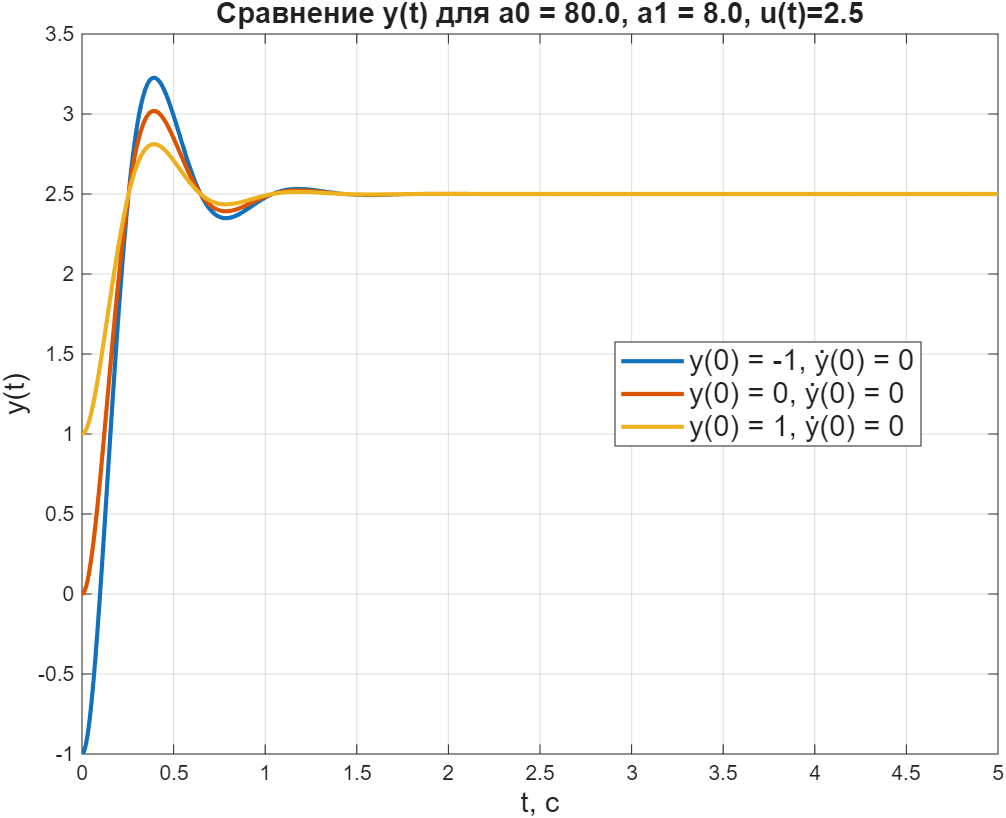
\includegraphics[width=0.65\linewidth]{images/Figure_3_1_1.png}
    \caption{График $y(t)$ для $a_0=80,\quad a_1=8, \quad u(t)=2.5$}
    \label{fig:placeholder}
\end{figure}

\begin{figure}[H]
    \centering
    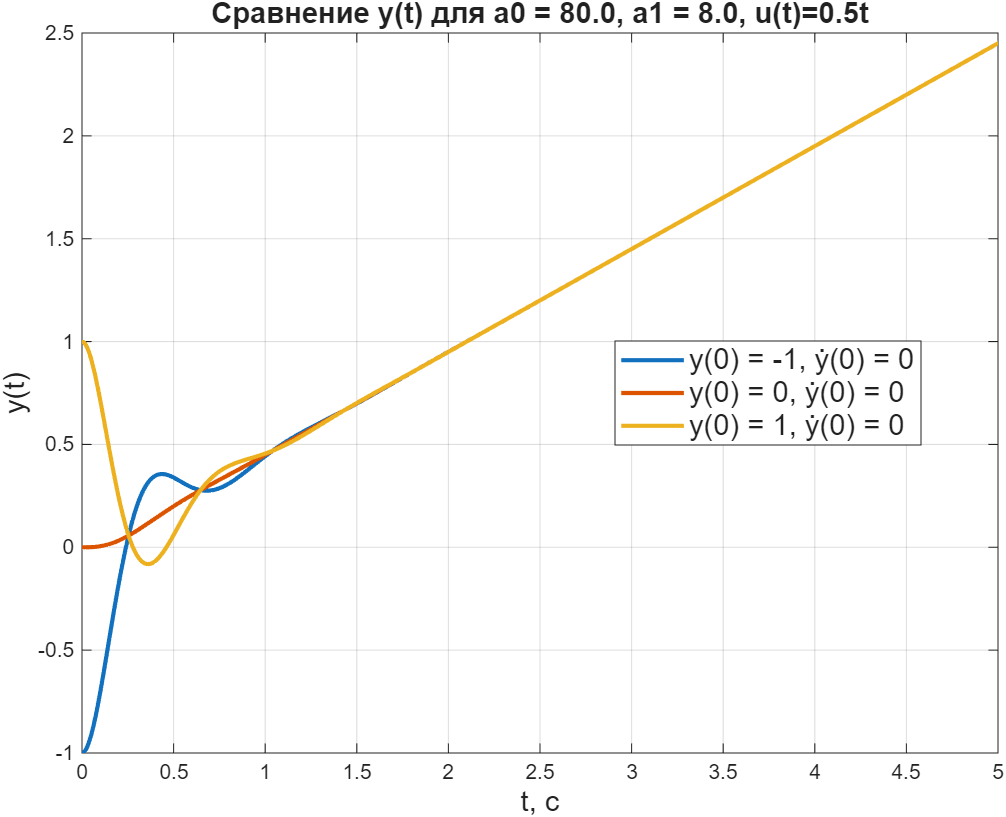
\includegraphics[width=0.65\linewidth]{images/Figure_3_1_2.png}
    \caption{График $y(t)$ для $a_0=80,\quad a_1=8, \quad u(t)=0.5t$}
    \label{fig:placeholder}
\end{figure}

\begin{figure}[H]
    \centering
    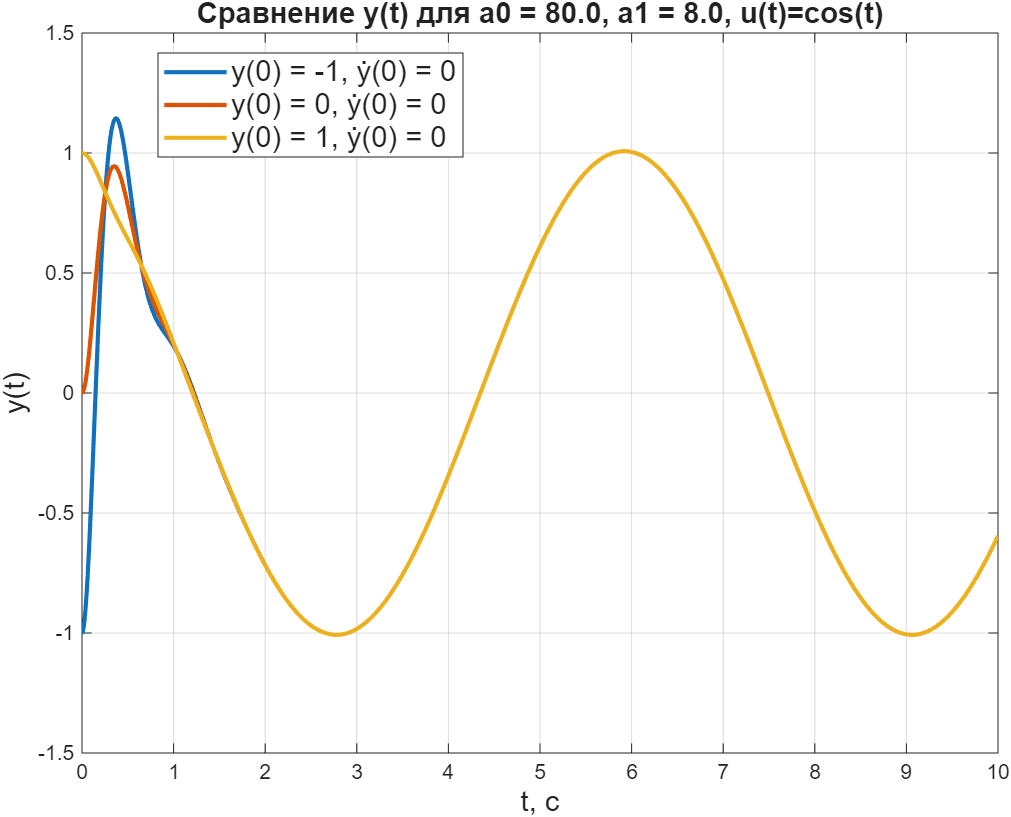
\includegraphics[width=0.65\linewidth]{images/Figure_3_1_3.png}
    \caption{График $y(t)$ для $a_0=80,\quad a_1=8, \quad u(t)=\cos t$}
    \label{fig:placeholder}
\end{figure}

\subsubsection{Системы на границе устойчивости}

\begin{figure}[H]
    \centering
    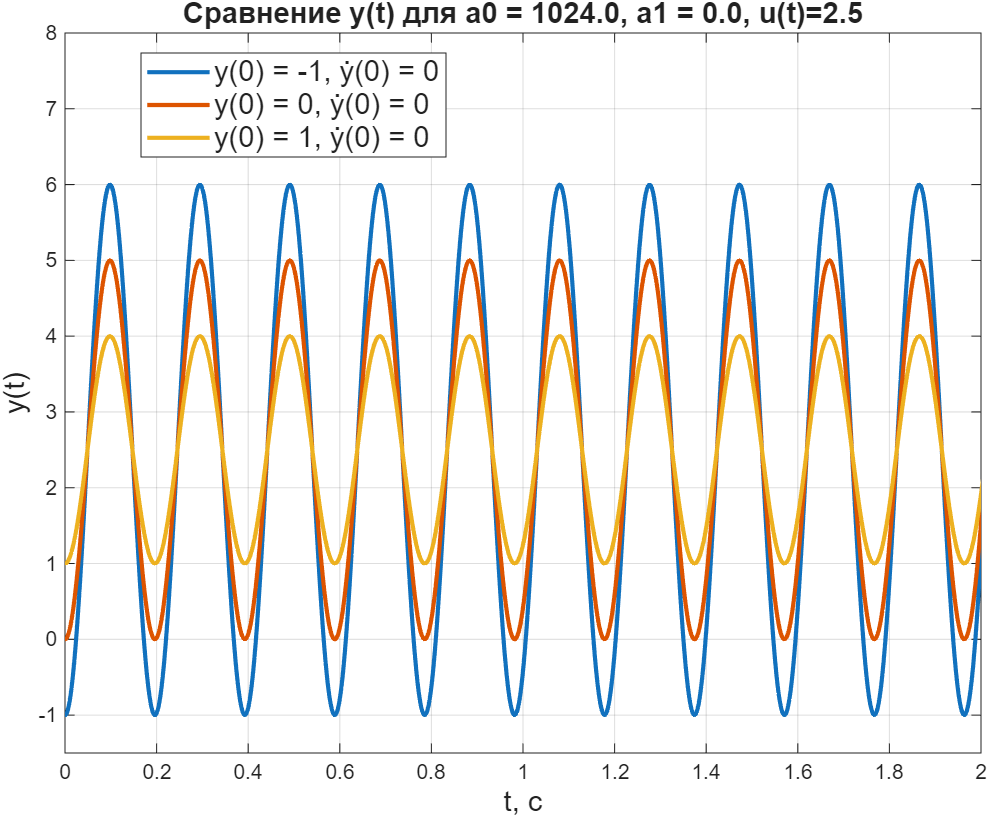
\includegraphics[width=0.65\linewidth]{images/Figure_3_1_4.png}
    \caption{График $y(t)$ для $a_1=0, \quad a_0=1024, \quad u(t)=2.5$}
    \label{fig:placeholder}
\end{figure}

\begin{figure}[H]
    \centering
    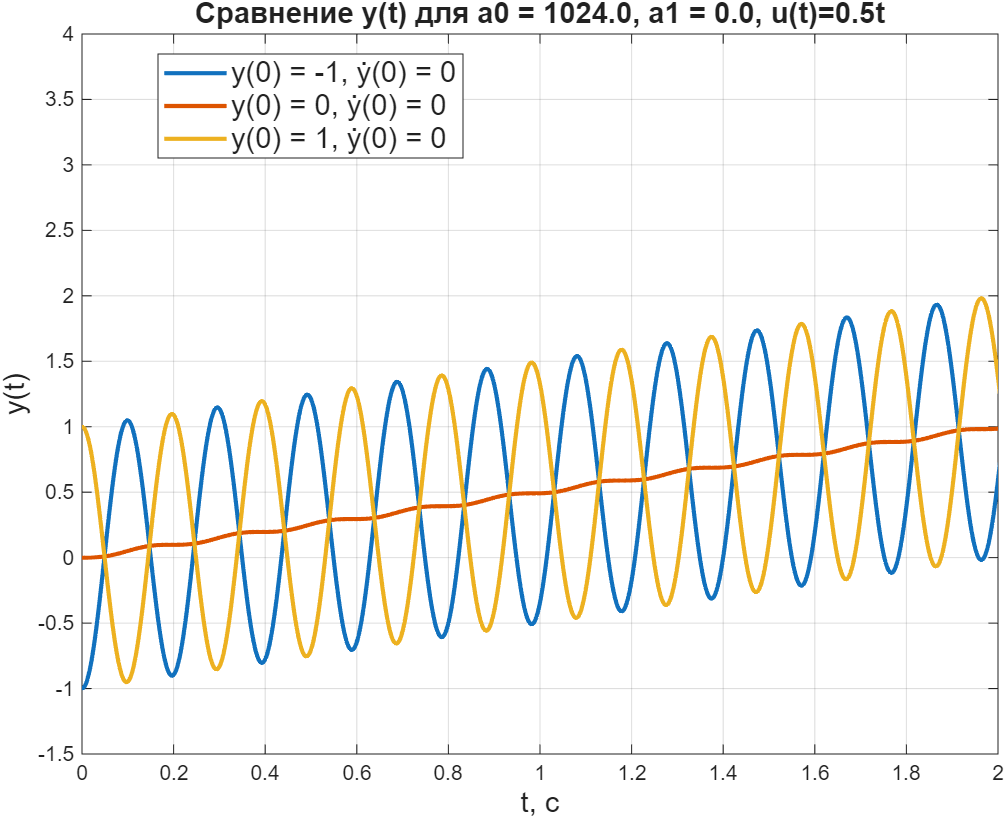
\includegraphics[width=0.65\linewidth]{images/Figure_3_1_5.png}
    \caption{График $y(t)$ для $a_1=0, \quad a_0=1024, \quad u(t)=0.5t$}
    \label{fig:placeholder}
\end{figure}

\begin{figure}[H]
    \centering
    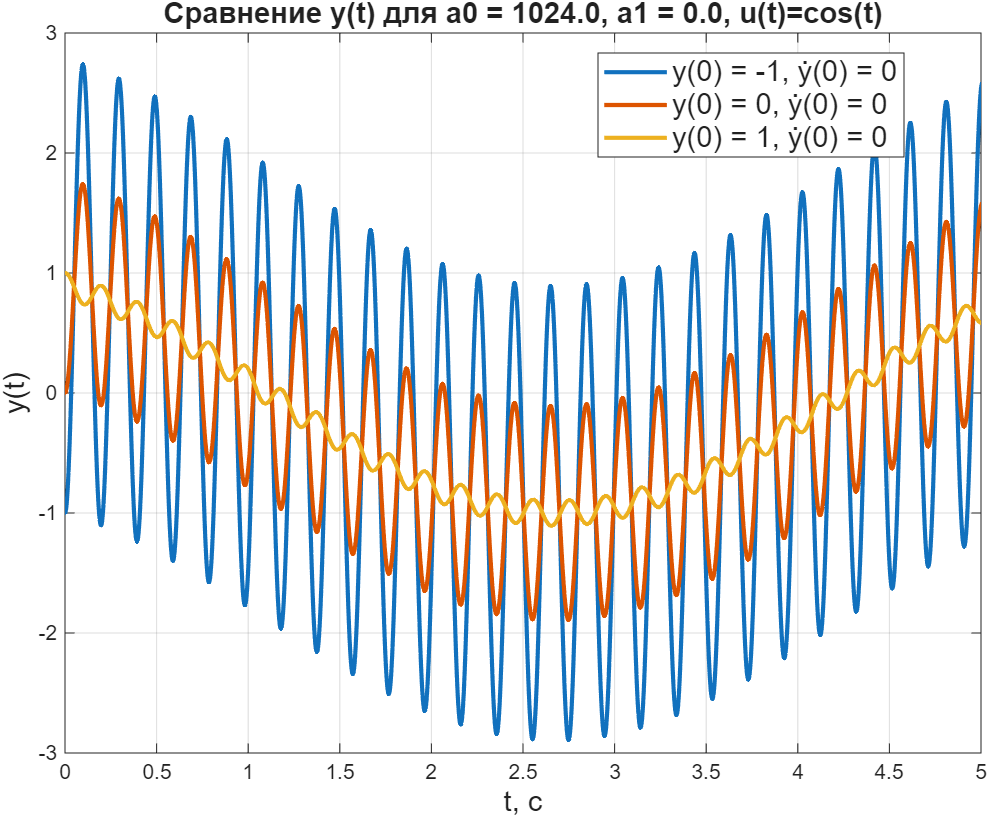
\includegraphics[width=0.65\linewidth]{images/Figure_3_1_6.png}
    \caption{График $y(t)$ для $a_1=0, \quad a_0=1024, \quad u(t)=\cos t$}
    \label{fig:placeholder}
\end{figure}

\subsubsection{Неустойчивые системы}

\begin{figure}[H]
    \centering
    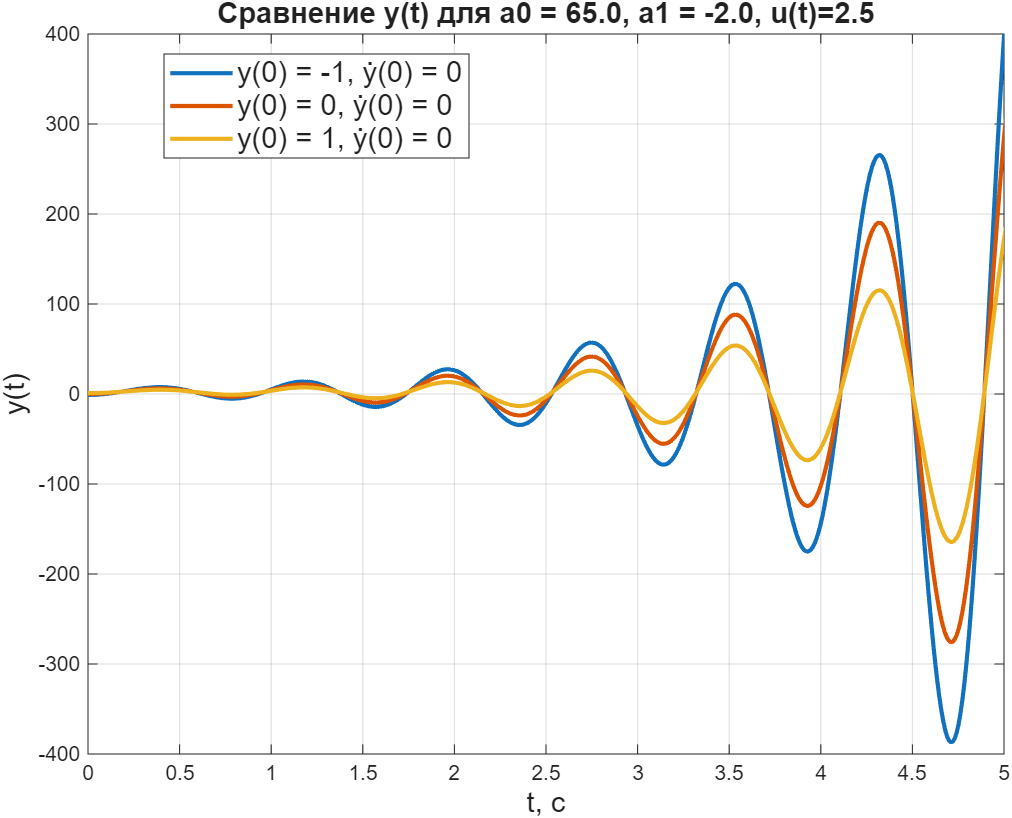
\includegraphics[width=0.65\linewidth]{images/Figure_3_1_7.png}
    \caption{График $y(t)$ для $a_1=-2, \quad a_0=65, \quad u(t)=2.5$}
    \label{fig:placeholder}
\end{figure}

\begin{figure}[H]
    \centering
    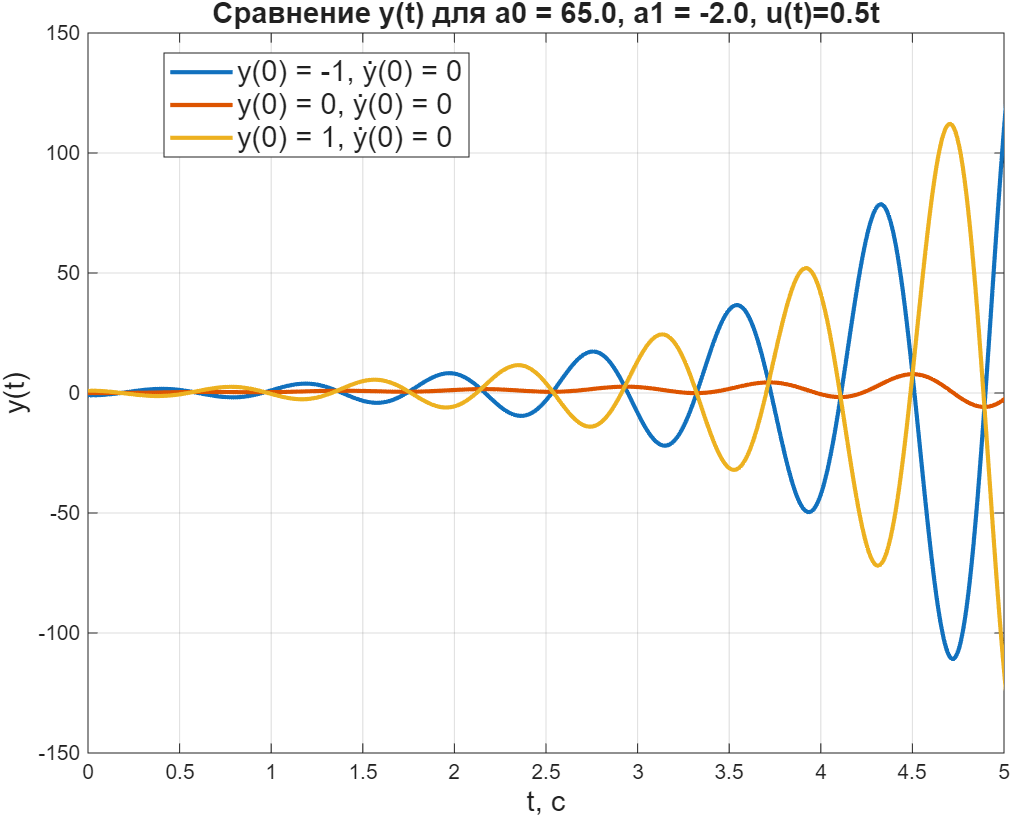
\includegraphics[width=0.65\linewidth]{images/Figure_3_1_8.png}
    \caption{График $y(t)$ для $a_1=-2, \quad a_0=65, \quad u(t)=0.5t$}
    \label{fig:placeholder}
\end{figure}

\begin{figure}[H]
    \centering
    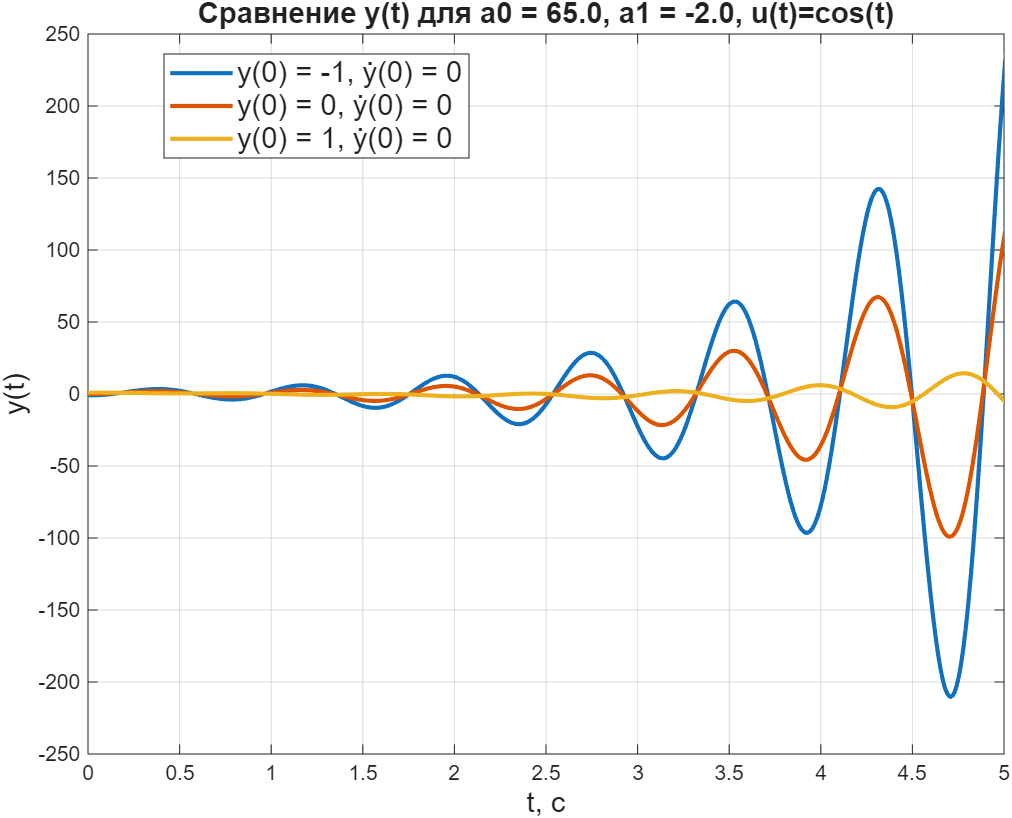
\includegraphics[width=0.65\linewidth]{images/Figure_3_1_9.png}
    \caption{График $y(t)$ для $a_1=-2, \quad a_0=65, \quad u(t)=\cos t$}
    \label{fig:placeholder}
\end{figure}

\subsection{Выводы}

Устойчивость системы определяется только коэффициентами $a_0$ и $a_1$. В устойчивой системе отклонения, вызванные начальными условиями, затухают, в системе на границе устойчивости сохраняются, а в неустойчивой системе со временем возрастают.

\subsubsection{Влияние начальных условий}

\textbf{Устойчивая система}\\
Начальные условия определяют только начальный участок движения системы. Переходная составляющая со временем затухает, и влияние начальных условий полностью исчезает, независимо от их величины.

\vspace{0.2cm}

\textbf{Система на границе устойчивости}\\
Начальные условия определяют амплитуду собственных колебаний системы и оказывают влияние на поведение выхода на всём интервале времени. При этом колебания не затухают, но и не усиливаются.

\vspace{0.2cm}

\textbf{Неустойчивая система}\\
В неустойчивой системе начальные условия определяют начальную амплитуду, при этом характер неограниченного роста определяется неустойчивыми полюсами системы.

\subsubsection{Влияние входных воздействий}

\textbf{Устойчивая система}\\
При различных начальных условиях выходные сигналы со временем сходятся к одному и тому же виду. В определенный момент поведение системы определяется только входным воздействием: при постоянном входе выход стремится к постоянному значению, при линейно возрастающем — повторяет характер роста входного сигнала, а при гармоническом воздействии воспроизводит его форму с ограниченной амплитудой.

\vspace{0.2cm}

\textbf{Система на границе устойчивости}\\
Система совершает незатухающие колебания вокруг зависимости, задаваемой входным воздействием.

\vspace{0.2cm}

\textbf{Неустойчивая система}\\
Любое входное воздействие приводит к неограниченному росту выходного сигнала. Амплитуда колебаний и значение выхода со временем увеличиваются

\section{Задание 2. Качество переходных процессов}

\subsection{Исходные данные}

Рассмотрим систему 3-го порядка, заданную передаточной функцией:

\begin{align}\label{du1}
    W(s)=\dfrac{|\lambda_1\lambda_2\lambda_3|}{(s-\lambda_1)(s-\lambda_2)(s-\lambda_3)}
\end{align}

Исследуем зависимости качества переходной характеристики от выбора полюсов передаточной функции.

\subsection{Выбор наборов полюсов}

\begin{table}[H]
\centering
\begin{tabular}{|c|c|}
\hline
№ набора & Полюса системы \\ \hline
1 & $\lambda_1=-2,\;\lambda_2=-3,\;\lambda_3=-4$ \\ \hline
2 & $\lambda_1=-2,\;\lambda_2=-3,\;\lambda_3=-6$ \\ \hline
3 & $\lambda_1=-1,\;\lambda_2=-3,\;\lambda_3=-4$ \\ \hline
4 & $\lambda_{1,2}=-2\pm 2j,\;\lambda_3=-3$ \\ \hline
5 & $\lambda_{1,2}=-2\pm 4j,\;\lambda_3=-3$ \\ \hline
6 & $\lambda_{1,2}=-2\pm 6j,\;\lambda_3=-4$ \\ \hline
\end{tabular}
\caption{Наборы полюсов исследуемых систем}
\label{tab:poles}
\end{table}

Степень колебательности будем считать по формуле:

$$
\mu=\max\left(\frac{|\operatorname{Im}\lambda_j|}{|\operatorname{Re}\lambda_j|}\right)
$$

Пререгулирование вычисляется по формуле:

$$
\sigma=\dfrac{|y_{\max}-y_{\text{уст}}|}{y_{\text{уст}}}
$$

Верхнюю оценку перерегулирования будем вычислять по формуле:

$$
\sigma \leq e^{-\frac{\pi}{\mu}} \cdot 100\%
$$

$$
\sigma_{\max} = e^{-\frac{\pi}{\mu}} \cdot 100\%
$$

Время перходного процесса $t_{\text{уст}}$ -- время, за которое выходной сигнал достигает и остается в зоне $\pm2\%$ от установившегося значения:

$$
|y(t)-y_{\text{уст}}|<0.2\cdot y_{\text{уст}}
$$

\begin{figure}[H]
    \centering
    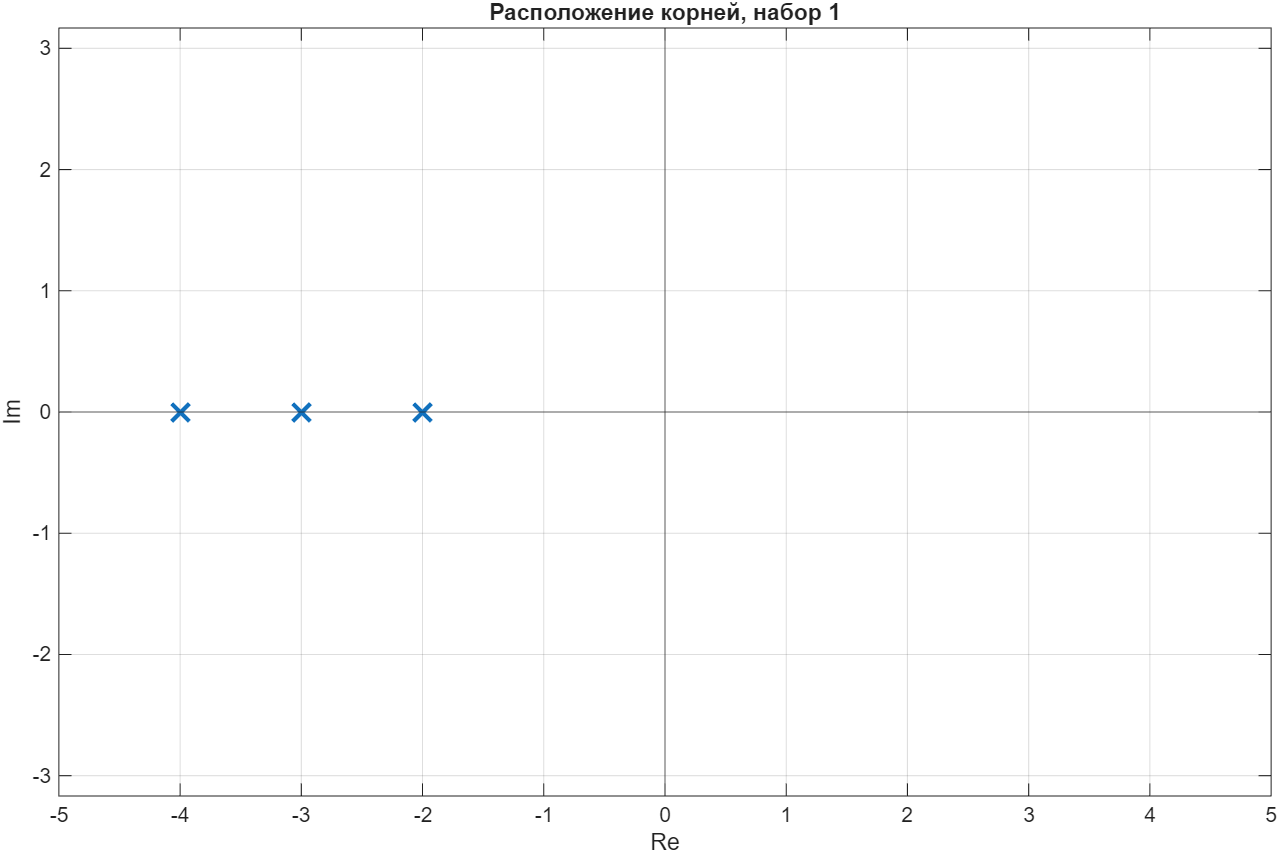
\includegraphics[width=0.7\linewidth]{images/Figure_3_2_1_1.png}
    \caption{Расположение полюсов (набор 1)}
    \label{fig:placeholder}
\end{figure}

\begin{figure}[H]
    \centering
    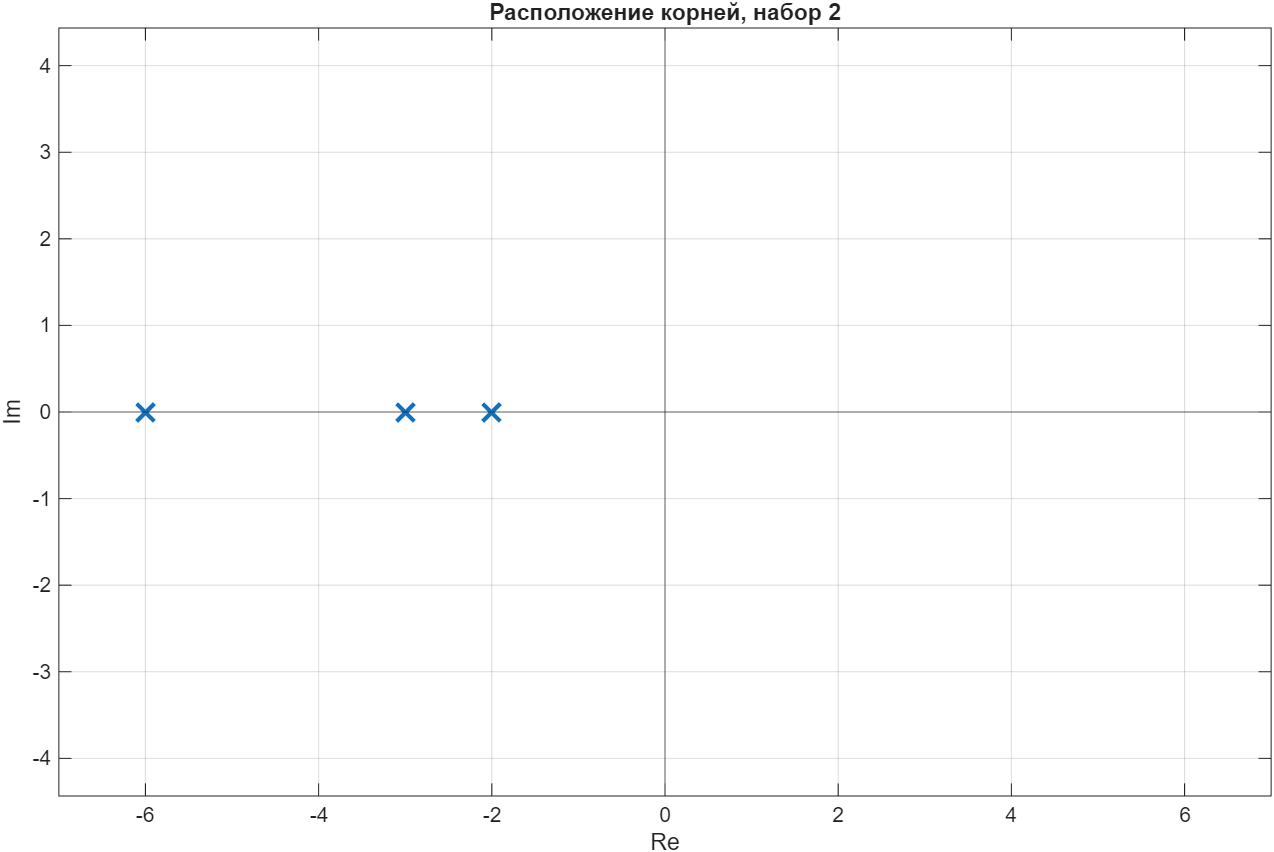
\includegraphics[width=0.7\linewidth]{images/Figure_3_2_1_2.png}
    \caption{Расположение полюсов (набор 2)}
    \label{fig:placeholder}
\end{figure}

\begin{figure}[H]
    \centering
    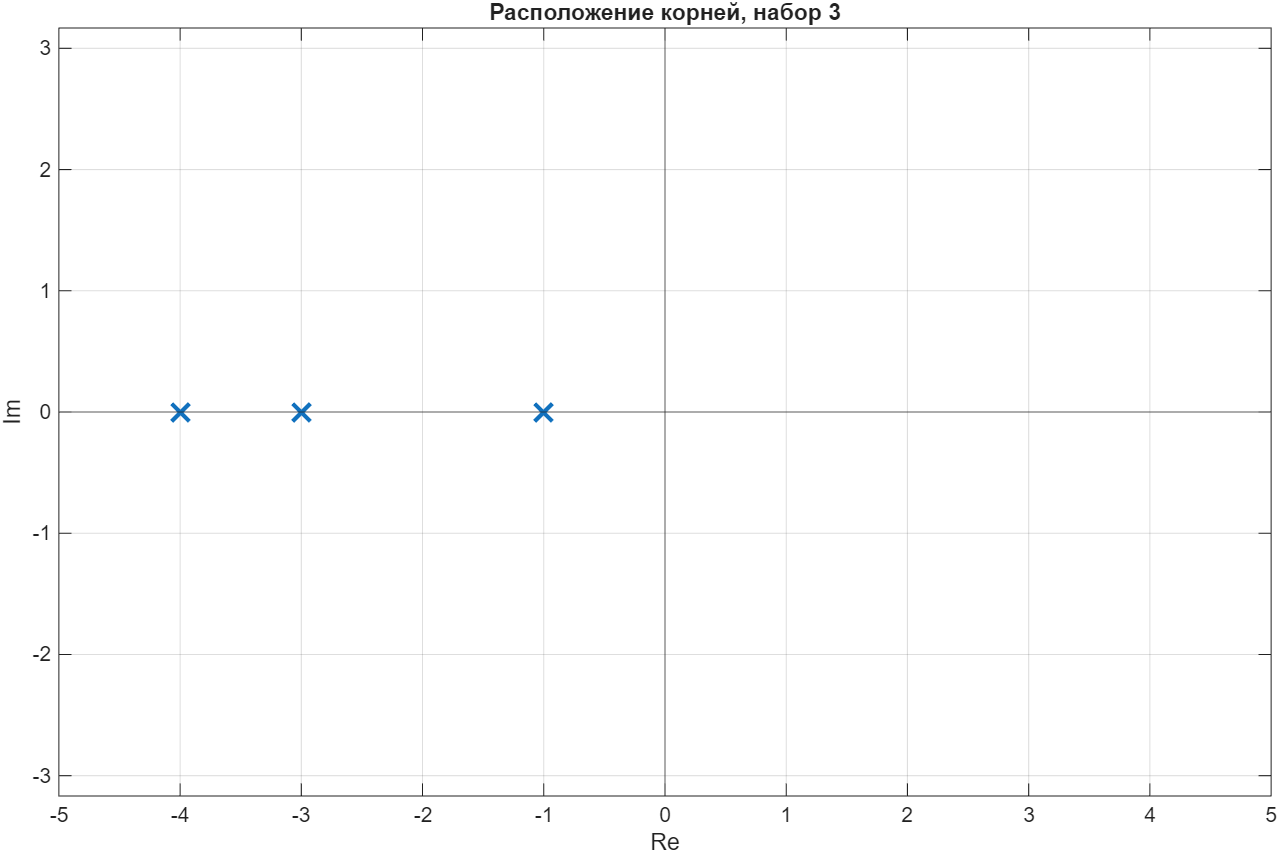
\includegraphics[width=0.7\linewidth]{images/Figure_3_2_1_3.png}
    \caption{Расположение полюсов (набор 3)}
    \label{fig:placeholder}
\end{figure}

\begin{figure}[H]
    \centering
    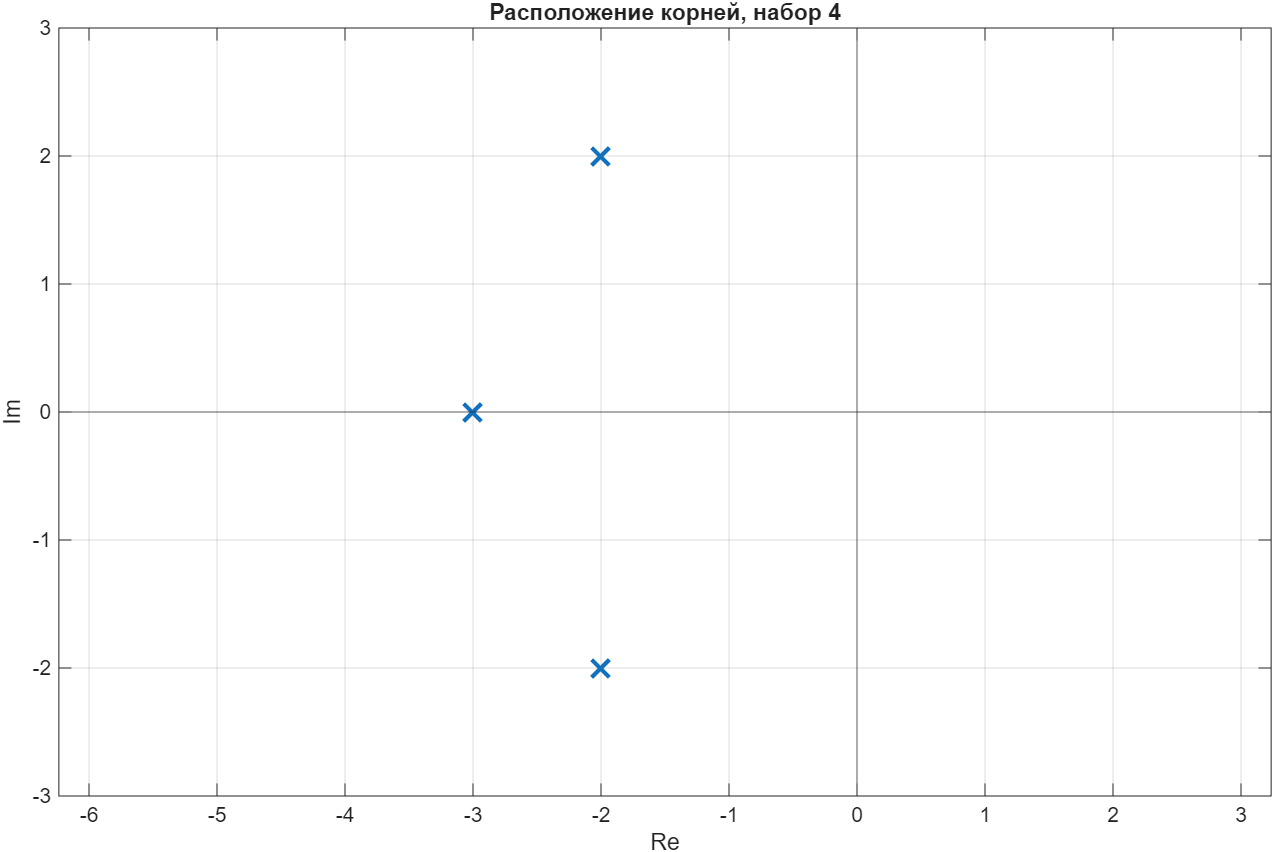
\includegraphics[width=0.7\linewidth]{images/Figure_3_2_1_4.png}
    \caption{Расположение полюсов (набор 4)}
    \label{fig:placeholder}
\end{figure}

\begin{figure}[H]
    \centering
    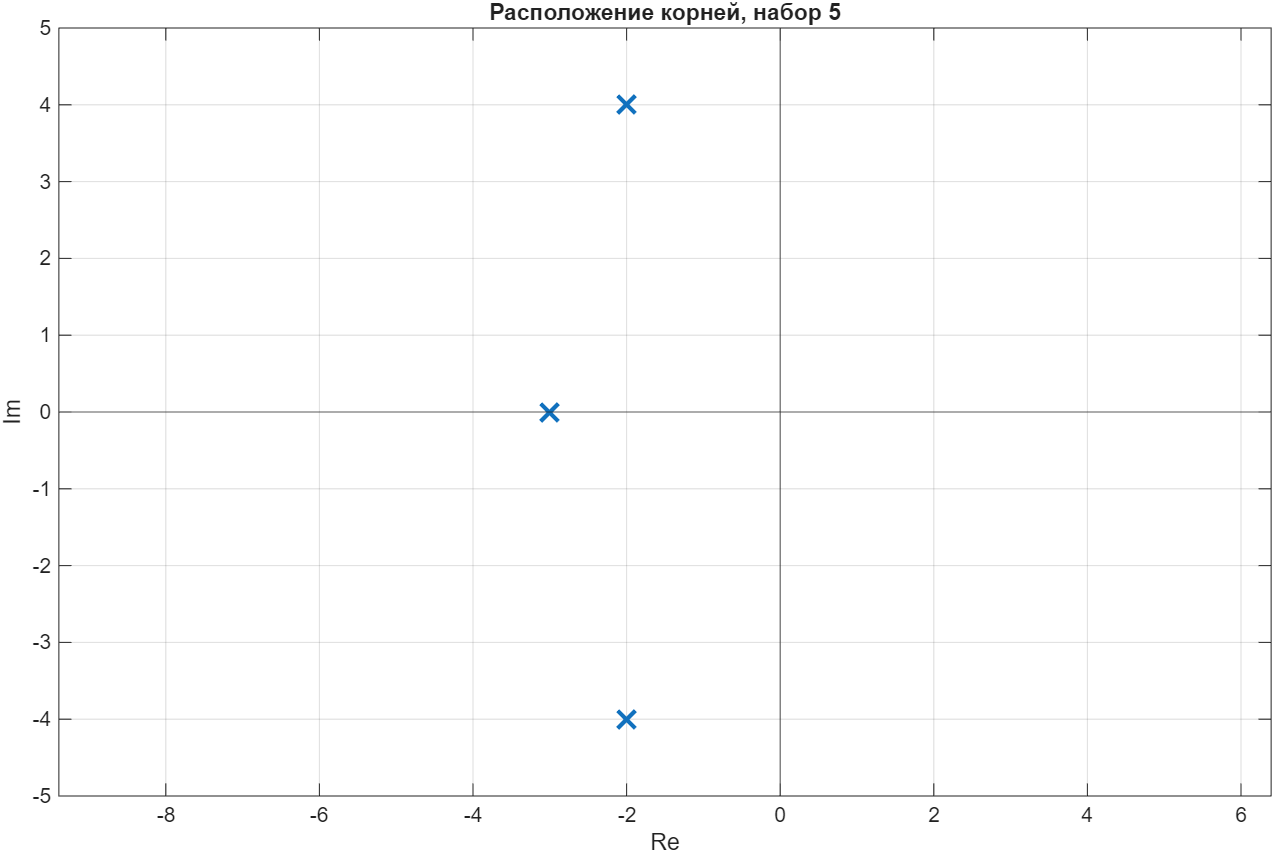
\includegraphics[width=0.7\linewidth]{images/Figure_3_2_1_5.png}
    \caption{Расположение полюсов (набор 5)}
    \label{fig:placeholder}
\end{figure}

\begin{figure}[H]
    \centering
    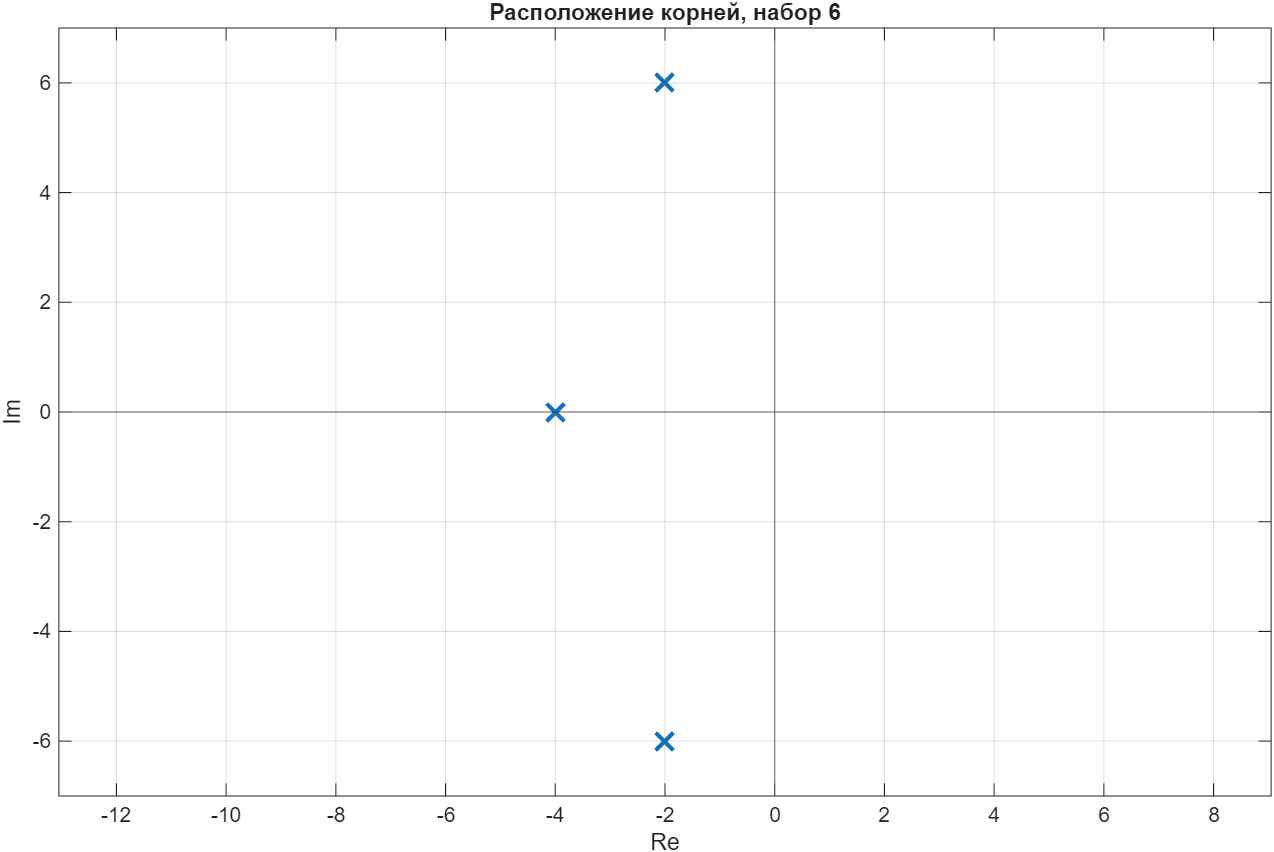
\includegraphics[width=0.7\linewidth]{images/Figure_3_2_1_6.png}
    \caption{Расположение полюсов (набор 6)}
    \label{fig:placeholder}
\end{figure}

\subsection{Графики переходных процессов}

\begin{figure}[H]
    \centering
    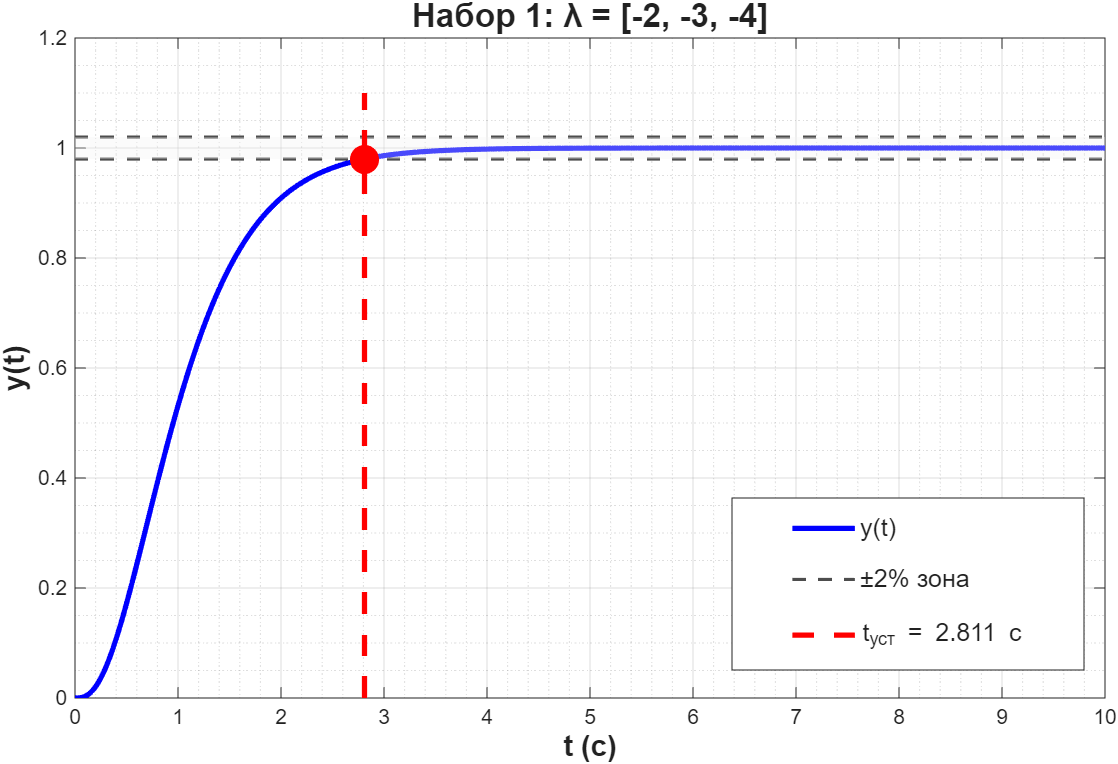
\includegraphics[width=0.7\linewidth]{images/Figure_3_2_2_1.png}
    \caption{Переходный процесс (набор 1)}
    \label{fig:placeholder}
\end{figure}

\begin{figure}[H]
    \centering
    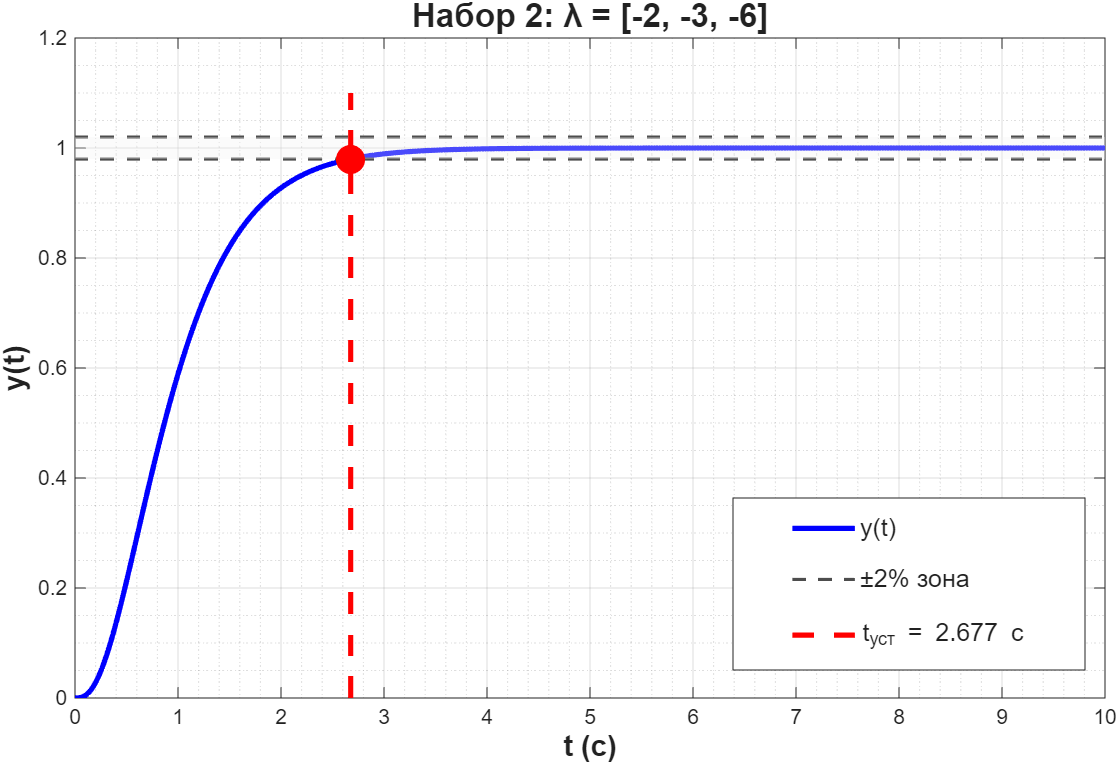
\includegraphics[width=0.7\linewidth]{images/Figure_3_2_2_2.png}
    \caption{Переходный процесс (набор 2)}
    \label{fig:placeholder}
\end{figure}

\begin{figure}[H]
    \centering
    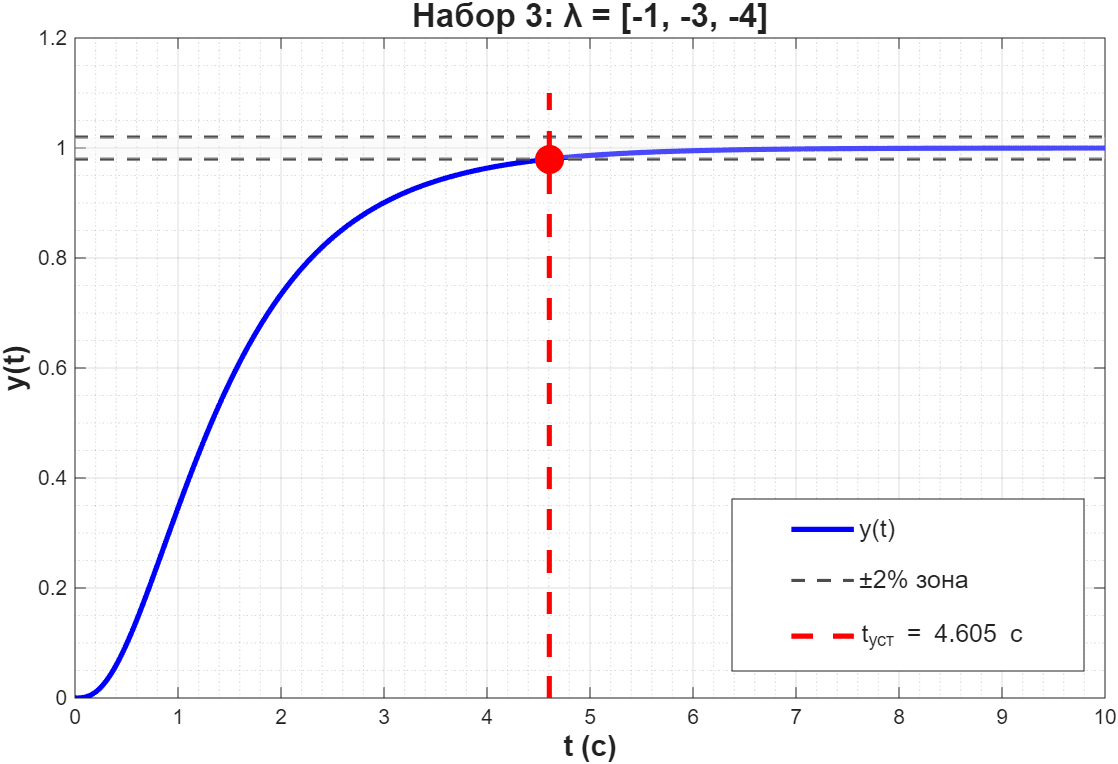
\includegraphics[width=0.7\linewidth]{images/Figure_3_2_2_3.png}
    \caption{Переходный процесс (набор 3)}
    \label{fig:placeholder}
\end{figure}

\begin{figure}[H]
    \centering
    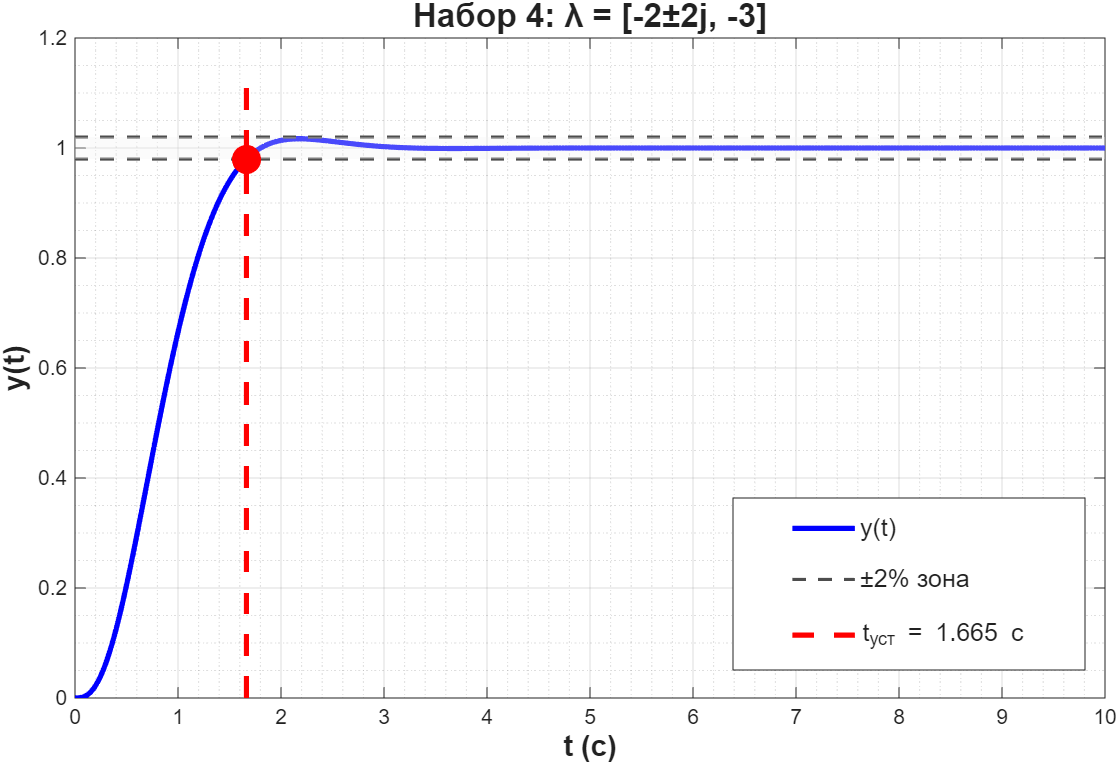
\includegraphics[width=0.7\linewidth]{images/Figure_3_2_2_4.png}
    \caption{Переходный процесс (набор 4)}
    \label{fig:placeholder}
\end{figure}

\begin{figure}[H]
    \centering
    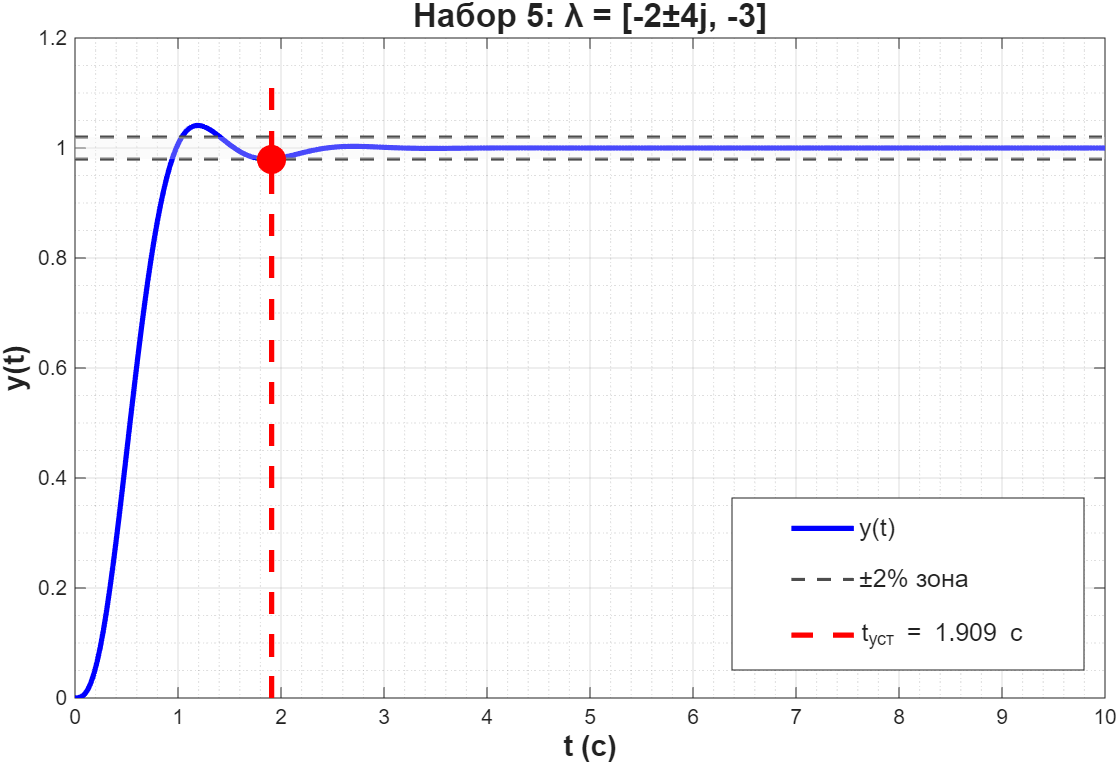
\includegraphics[width=0.7\linewidth]{images/Figure_3_2_2_5.png}
    \caption{Переходный процесс (набор 5)}
    \label{fig:placeholder}
\end{figure}

\begin{figure}[H]
    \centering
    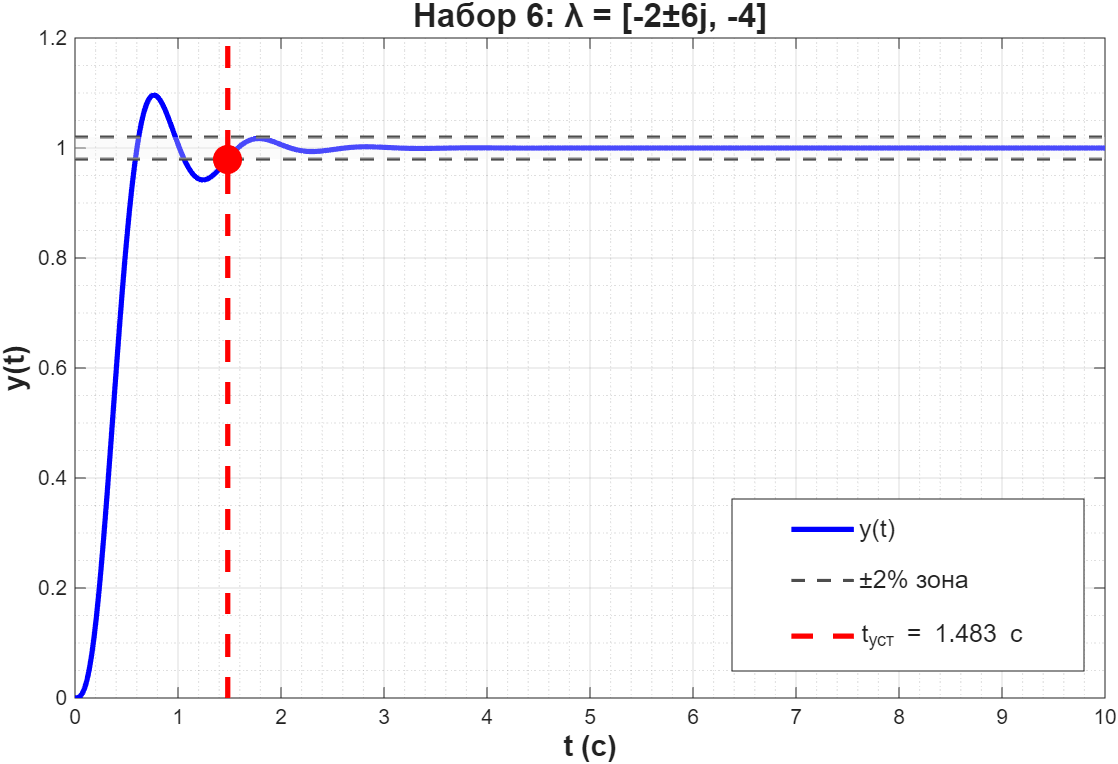
\includegraphics[width=0.7\linewidth]{images/Figure_3_2_2_6.png}
    \caption{Переходный процесс (набор 6)}
    \label{fig:placeholder}
\end{figure}

\subsection{Полученные значения}

\begin{table}[H]
\centering
\begin{tabular}{|c|c|c|c|c|c|}
\hline
№ набора & Полюса системы & $\mu$ & $\sigma$ & $\sigma_{\max}$ & $t_{\text{уст}}$ \\ \hline
1 & $\lambda_1=-2,\;\lambda_2=-3,\;\lambda_3=-4$ & 0 & 0 & - & 2.811 \\ \hline
2 & $\lambda_1=-2,\;\lambda_2=-3,\;\lambda_3=-6$ & 0 & 0 & - & 2.677 \\ \hline
3 & $\lambda_1=-1,\;\lambda_2=-3,\;\lambda_3=-4$ & 0 & 0 & - & 4.605 \\ \hline
4 & $\lambda_{1,2}=-2\pm 2j,\;\lambda_3=-3$ & 1 & 1.663 & 4.321 & 1.665 \\ \hline
5 & $\lambda_{1,2}=-2\pm 4j,\;\lambda_3=-3$ & 2 & 4.107 & 20.788 & 1.909 \\ \hline
6 & $\lambda_{1,2}=-2\pm 6j,\;\lambda_3=-4$ & 3 & 9.635 & 35.092 & 1.483 \\ \hline
\end{tabular}
\caption{Полученные значения $\mu$, $\sigma$, $t_{\text{уст}}$ для 6 наборов $\lambda_{123}$}
\label{tab:poles}
\end{table}

\subsection{Выводы}

Для наборов с исключительно вещественными отрицательными полюсами (1-3 наборы) переходные процессы апериодические и монотонные, без перерегулирования, при этом время установления увеличивается при уменьшении модуля произведения полюсов и наоборот.

Для систем с комплексно-сопряжёнными полюсами (4-6 наборы) наблюдается колебательный характер переходного процесса. Увеличение мнимой части полюсов приводит к росту степени колебательности и перерегулирования.

\section{Выводы}
В ходе выполнения лабораторной работы были исследованы вынужденные движения линейных систем и показатели качества переходных процессов. В первом задании было показано, что устойчивость системы существенно влияет на характер её реакции: в устойчивых системах влияние начальных условий со временем исчезает, а выходной сигнал определяется только входным воздействием; на границе устойчивости сохраняются незатухающие колебания; в неустойчивых системах наблюдается неограниченный рост выходной величины. Также установлено, что вид входного сигнала определяет форму установившегося режима системы.

Во втором задании была проанализирована зависимость качества переходного процесса от расположения полюсов передаточной функции. Выявлено, что системы с вещественными отрицательными полюсами обладают апериодическим и монотонным переходным процессом без перерегулирования, а наличие комплексно-сопряжённых полюсов приводит к колебательному характеру переходного процесса. Увеличение мнимой части полюсов вызывает рост степени колебательности и перерегулирования, при этом время установления может уменьшаться.

Таким образом, в работе наглядно подтверждена связь между параметрами системы, её устойчивостью и показателями качества, а также продемонстрирована возможность управления динамическими свойствами системы путём выбора расположения полюсов.


\end{document}